\normaltrue \difficilefalse \tdifficilefalse
\correctionfalse

%\UPSTIidClasse{11} % 11 sup, 12 spé
%\newcommand{\UPSTIidClasse}{11}

\exer{Axe de commande $\star$ \label{G2:01:2002}}
\setcounter{question}{0}\UPSTIcompetence[2]{G2-01}
\index{Compétence G2-01}

\ifcorrection
\else
\marginnote{\textbf{Pas de corrigé pour cet exercice.}}
\fi


\ifprof 
\else
Soit la pièce suivante.
\begin{center}
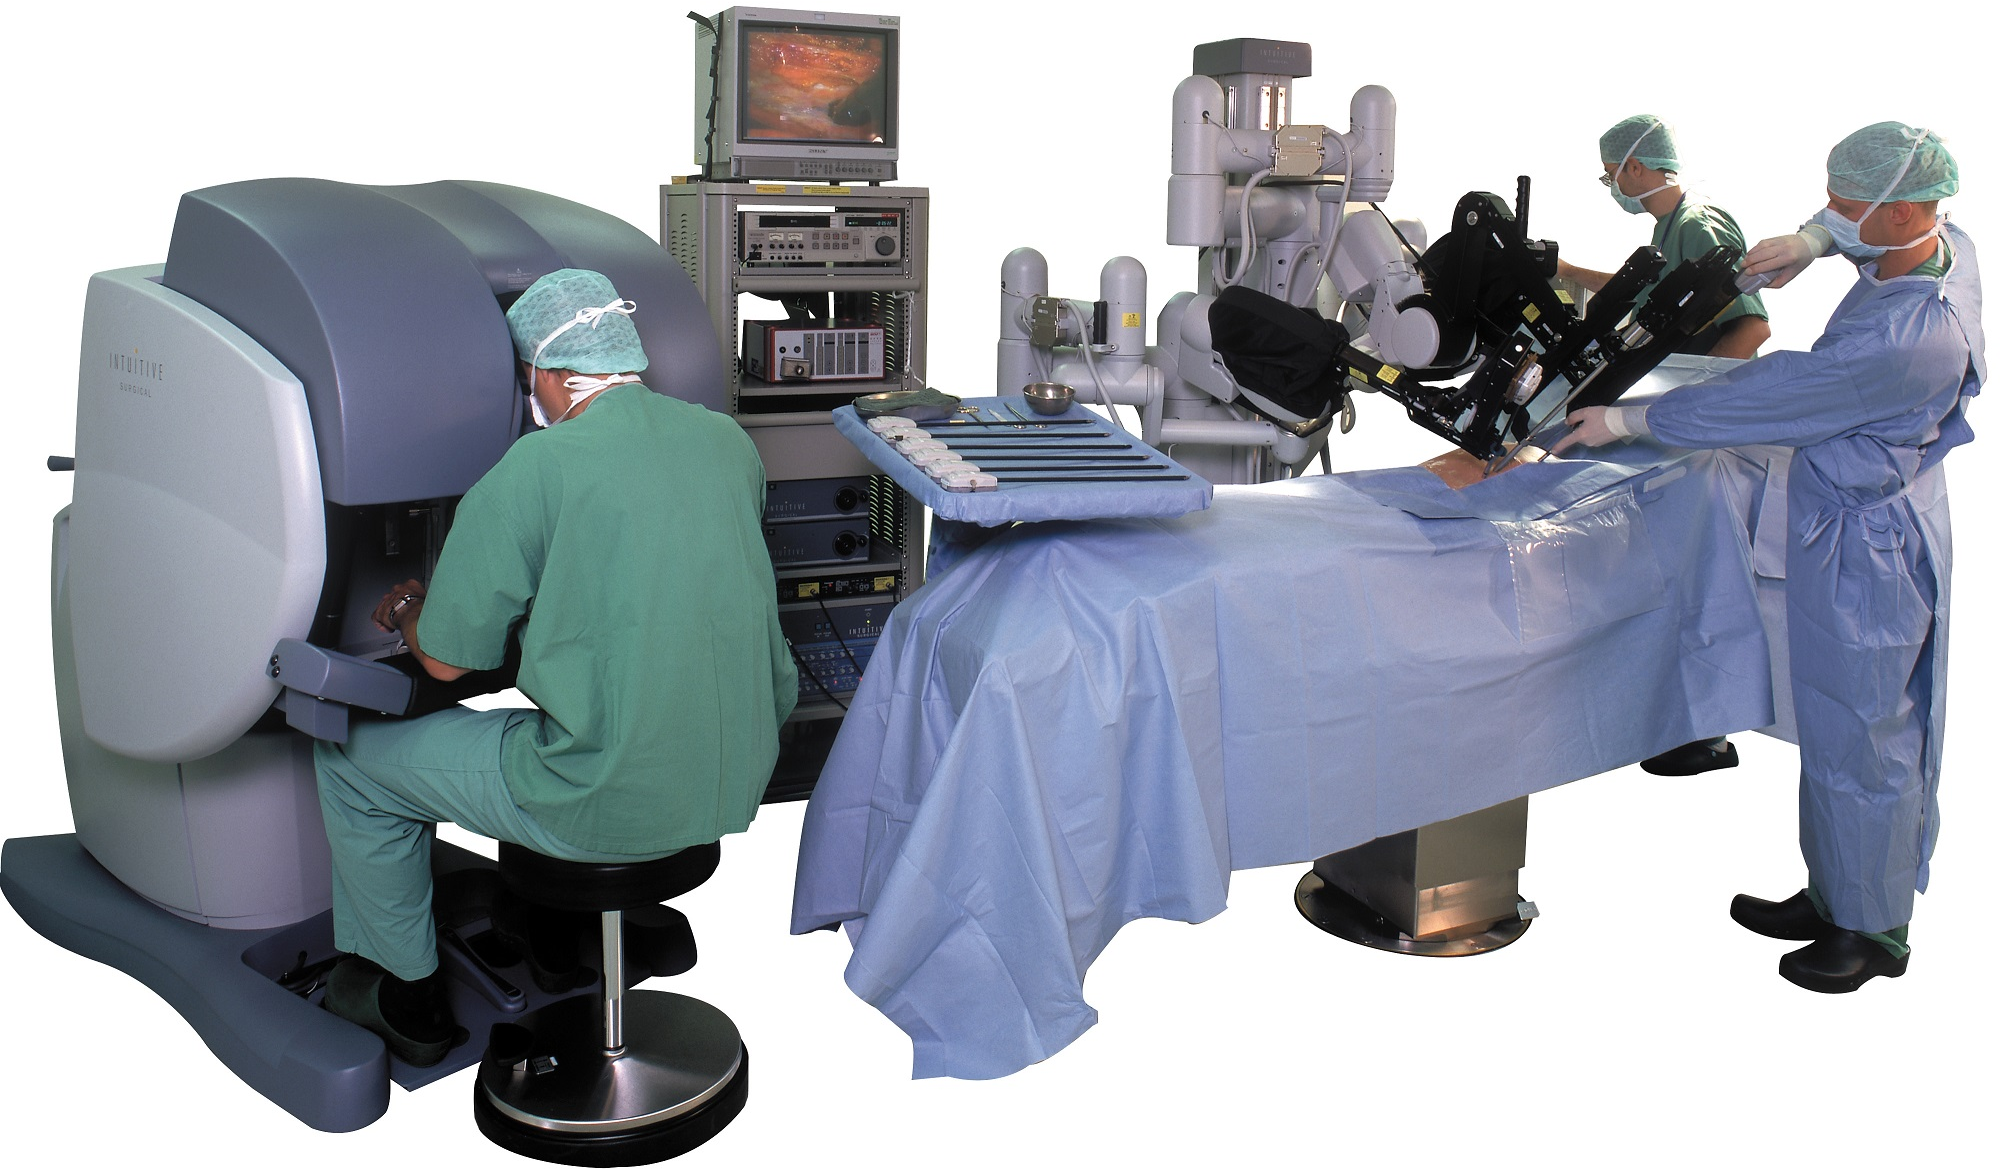
\includegraphics[width=.9\linewidth]{fig_01}
\end{center}
 \fi
 
\question{Proposer une gamme de fabrication, de l'élaboration du brut à la finition.}
\ifprof
\begin{center}
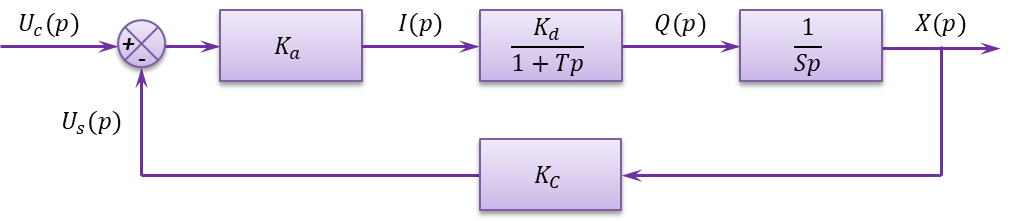
\includegraphics[width=.9\linewidth]{cor_01}
\end{center}

\else 
\fi

Avant usinage de la pièce, une simulation a été réalisée pour voir les contraintes et déplacements engendrés sur la pièce. 

\begin{center}
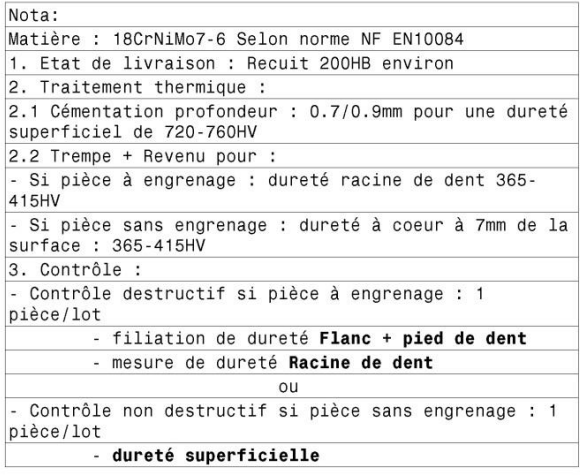
\includegraphics[width=.9\linewidth]{fig_02}
\end{center}

\question{La pièce a été réalisée en acier. Qu'est-ce qu'un acier ? Qu'est-ce qu'une fonte ?}

\question{La limite d'élasticité est de \SI{800}{Mpa}. Que cela signifie-t-il ? Détailler l'essai permettant d'obtenir cette valeur.}


\ifprof
\else
\begin{flushright}
\footnotesize{Corrigé  voir \ref{G2:01:2002}.}
\end{flushright}%
\fi